% Overall overview of the adopted user testing procedure
\section*{User Testing}

\subsection{General Method}
The core of User Testing is to assess the usability properties of a system by observing how the system is used by users that are representative of real end users. It is a form of empirical research that aims to understand the relationship between humans and technology, learning how humans interact with a designed system through observed phenomena. 
Users are assigned pre-defined tasks to complete using the system and are then observed, recorded and finally analysed. 
Through user testing we can uncover actual difficulties that users will face, ones perhaps overlooked during the initial design of the system .

\subsection{Design Of The Study}
The User Testing study was designed to give probable users tasks that they would likely need to use the UNICEF website for. Moreover, as User Testing was performed after the Inspection testing of the website, the tasks were modelled to investigate further issues that were previously found. 

The user profile used for recruiting users was aimed at an age range of 20 to 35 as the average age of UNICEF volunteers is reported to be 34. Due to this age range’s familiarity with websites and technology in general, the tasks we designed to push their abilities.

After the initial inspection, it was discussed and agreed that the primary actions that a user can use the website for are:
\begin{itemize}
    \item To donate money 
    \item Research information
    \item Volunteer with the charity
    \item Find contact information
    \item Find the charity’s social media accounts
  \end{itemize}

  With each of these actions the quality of the site is not only tested by achieving the desired outcome for each task but also with what ease and efficiency can the user complete each action. 
  With each task the user is provided brief context and motivation for the action they need to preform. 

\begin{itemize}
    \item [A] Task: You would like to support UNICEF in their work 
    Make a once off donation of €10 euro to the charity 
    Stop this task before confirming payment.
    \item [] Motivation: As UNICEF is a charity organisation, a primary goal of their website is to fundraise money. For this reason the action of donation is essential to the success of the website. 

    \item[B] Task: Your manager at work has a letter that must be sent to the ethic’s office of UNICEF 
    Find the appropriate postal address that this letter should be sent to
    
    \item[] Motivation: A primary action on a website of this kind is finding relevant contact information. After inspecting the website, we chose to ask for the Ethic’s Office postal address specifically as it’s location is not obvious, and so would be a greater test of our technologically apt test group. 

    \item[C] Task: From what you have read on the UNICEF website you are very interested in their work and you would like to be kept up to date with any news from the organisation
    Find a way to subscribe to new information or updates from UNICEF

    \item[] Motivation: Getting users to subscribe to information updates is a useful tool for organisations such as UNICEF.
    
    \item[D] Task: You are interested in working with UNICEF either as an intern or as a volunteer
    Find what opportunities are available
    \item[] Motivation: For a charity as large as UNICEF, finding new volunteers and employees is essential. We were also interested to see how users felt navigating these sections due to the large amount of information available. 
    
    \item[E] Task: For a university project, you have been asked to write about the impact of charity work on Women’s Rights in Africa
    You decide to do some research on the UNICEF website.
    Find out some information on the work the organisation does to help women in Africa. 
    \item[] Motivation: As already mentioned, a primary use of the website is for users to gather information on social issues and the work UNICEF does to help them. The task specified the information that needed to be found in order to see would users use the search feature or other methods. 

    \item[F] Task: You have recently become a parent. 
    Find the area of the website with the relevant information about this topic and sign up.
    \item[] Motivation: This tas was chosen due to the action needing to be performed only being possible in one specific location. 
    
\end{itemize}

\subsection{Execution of The Study}


The testing was kept as uniform as possible across all users. With the exception of X-many using the mobile version of the website and X-many doing the testing remotely. 

First the users were given an explanation of the testing with relevant guidelines and rules.  

Next the users were given a google form to fill out prior to starting the tasks. The form, shown below, recorded the user’s age, highest level education and some other general background data. The purpose of gathering this information is that it could possibly be later used to explain deviations in users’ success with the tasks.
\begin{figure}[h]
    \centering
    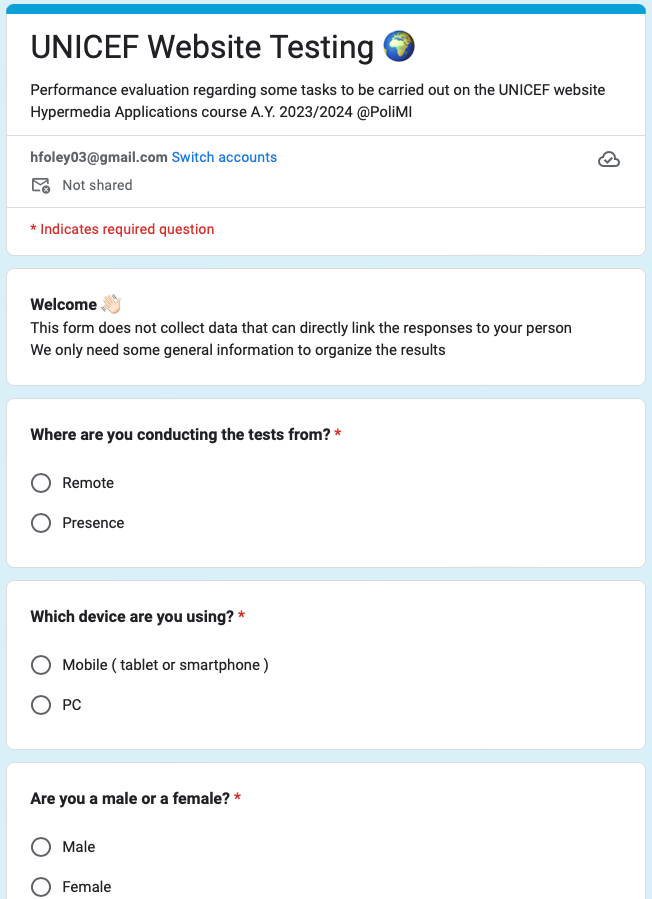
\includegraphics[scale=0.5]{Resources/Harry/GoogleForm.png}
    \caption{A section of the Google Form used for User Testing}
\end{figure}
It was decided to given minimal help to the users during testing to closer simulate the actual end users experience.

A specific time limit was formulated for each task, with a user’s time exceeding this being considered a fail. However, users would not be told that they had failed a task if they exceeded the limit, as to not discourage them. This also allowed us to maximise the amount of information gathered during the study. The time limits were found through dummy testing with users not considered by the study. 

After the users had completed all tasks, they were asked to describe their experience, highlighting anything they found enjoyable or frustrating. 


